\documentclass[../main.tex]{subfiles}

\begin{document}

\renewcommand{\labelitemi}{\ding{226}}
\renewcommand{\labelitemii}{\ding{227}}

\part{The T2K experiment}
\label{T2K:general}

\chapter{Neutrino beam}
\label{T2K:nu_beam}
\chapter{Near detector}
\label{T2K:nd}
\section{Near detector ND280}
\label{T2K:nd280}
\begin{figure}[h!]
    \begin{center}
    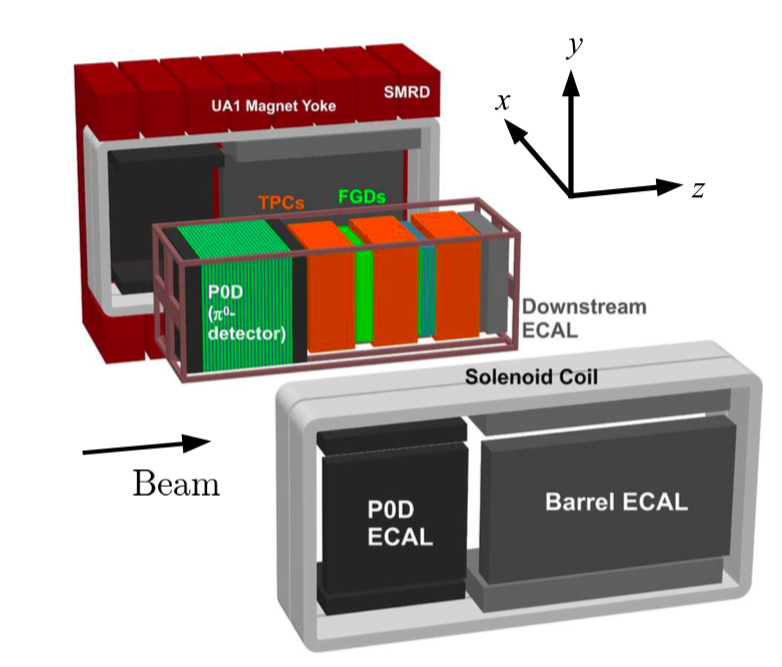
\includegraphics[width = 0.7\linewidth]{ND280}
    \caption{An exploded view of the ND280 off-axis detector.}
    \label{T2K:fig:ND280}
    \end{center}
\end{figure}
\subsection{Time projection chambers (TPC)}
\subsubsection{TPC concept}
\subsection{Fine grained detectors (FGD)}
\subsection{Electromagnetic calorimeter (ECaL)}
\section {INGRID}
\chapter{SuperKamiokande}
\chapter{Analysis overview}
\section{Neutrino flux measurements}
\section{Neutrino cross-section measurements}
\section{Oscillation analysis}
\end{document}